\documentclass[12pt]{article}


\usepackage[utf8]{inputenc}
\usepackage[a4paper,top=3cm,bottom=2cm,left=3cm,right=3cm,marginparwidth=1.75cm]{geometry}
\usepackage[nodayofweek]{datetime}
\usepackage{tabularx}
\usepackage[small]{titlesec}
\usepackage{graphicx}
\usepackage{tabularx}

\newcolumntype{L}[1]{>{\raggedright\arraybackslash}p{#1}}
\newcolumntype{C}[1]{>{\centering\arraybackslash}p{#1}}
\newcolumntype{R}[1]{>{\raggedleft\arraybackslash}p{#1}}

\begin{document}

\begin{titlepage}
    \begin{center}
        \huge{\bfseries  Tribhuvan University}\\
        \Large{Institute of Engineering}\\
        \huge{ \bfseries  Pulchowk Campus}\\[3.2cm]


        \textsc{\Large Big Data Technologies}\\[-0.5cm]
        \line(1,0){400}\\
        \huge{\bfseries Project Report}\\
        \Large{\bfseries Restaurant Finder\\}
        \line(1,0){400}\\


        \textsc{\Large Submitted by:}\\
        \Large Aayush Lamichhane\\ \large 075BCT005\\    [0.85cm]
        \Large Bishal Katuwal\\ \large 075BCT028\\    [0.85cm]
        \Large Bishant Baniya\\ \large 075BCT030\\    [0.85cm]
        \Large Gobind Pd Sah\\ \large 075BCT038\\    [0.85cm]


        \textsc{\Large Submitted to:}\\\
        \large Department of Electronics and Computer Engineering\\Pulchowk Campus\\    [0.85cm]
        
        \textsc{\Large Submitted on:}\\
        \today
        
    \end{center}
\end{titlepage}
\pagebreak
\tableofcontents
\pagebreak
\listoffigures
\pagebreak
\listoftables
\pagebreak
% ===============================================================
\section{Introduction}
\subsection{Background}
The purpose of this project is to create a restaurant finder application that allows users to search for restaurants by cuisine using Elasticsearch. The application retrieves data from a MongoDB database and transforms it to be indexed into Elasticsearch. Users can then input a cuisine type into the search bar and the application will return a list of restaurants matching the search criteria.
\subsection{Problem Statement}
Finding a restaurant that serves a specific cuisine can be time-consuming and difficult, especially in a large city with many dining options. The goal of this project is to create a web-based application that allows users to search for restaurants based on cuisine type and location, and view the results in a user-friendly format.

\section{Technologies used}
The project relies on two primary technologies: MongoDB and Elasticsearch. 
\subsection{MongoDB}
MongoDB is a NoSQL document-oriented database. It is designed to store data in JSON-like documents, making it easy to store and retrieve data from the database. MongoDB is highly scalable and can handle large volumes of data. In this project, MongoDB is used to store data about restaurants, including their names, cuisines, and addresses.
\subsection{ElasticSearch}
ElasticSearch is an open-source, distributed search engine. It is based on the Lucene library and provides full-text search capabilities. ElasticSearch is highly scalable and can handle large volumes of data. It is commonly used for logging, monitoring, and analytics. Elasticsearch is used in this project to index and search through the restaurant data stored in MongoDB, and to return relevant search results based on the user's input.
\subsection{Flask}
Flask is a lightweight web framework for Python. It is used to build web applications quickly and easily. Flask is flexible and allows developers to customize it to their needs. It provides support for various extensions that can be used to add additional functionality. The web-based application is built using the Flask web framework. The application allows users to search for restaurants based on cuisine type and location, and returns results in a user-friendly format that includes the name, cuisine, address, and borough of each restaurant. 
\subsection{HTML/CSS}
HTML is a markup language used to create web pages. It defines the structure and content of the page. CSS is a style sheet language used to add style and formatting to web pages. It defines the presentation of the page, including layout, colors, fonts, and more. Together, HTML and CSS are used to create visually appealing and functional web pages. Our application also includes a front-end interface that allows users to input their search criteria and view the results in real-time.


\section{Methodology}
The application is built using Python Flask Framework, which allows for easy integration with Elasticsearch and MongoDB. A MongoDB database was used to store the restaurant data, which was then transformed to be indexed into Elasticsearch.

The Elasticsearch index was created from Mongo BD with the following mapping properties: "name", "address", "cuisine", "borough". The "address" field contains sub-properties for "building", "coord", "street", "zipcode", and "borough".

When a user inputs a cuisine type into the search bar, the application queries Elasticsearch for restaurants matching the search criteria. The results are then displayed on a search results page in an HTML template.

The HTML templates were designed to be simple and user-friendly. The home page displays a search bar for the user to input their search criteria. The search results page displays the restaurant results in a clean, organized manner. The HTML templates were styled using CSS to improve the visual appearance of the pages.

\section{Code}
\begin{verbatim}
from flask import Flask, request, render_template, jsonify,url_for,redirect
from pymongo import MongoClient
from elasticsearch import Elasticsearch

# Set up MongoDB client

connection_string = STRING HERE'
mongo_client = MongoClient(connection_string)
mongo_db = mongo_client['sample_restaurants']
mongo_collection = mongo_db['restaurants']

# # Set up Elasticsearch client
es_client = Elasticsearch(
    hosts=[{'host':'localhost','port':9200,'scheme':'https'}],
    basic_auth= ('USERNAME','PASSWORD'),
    verify_certs=False)
index_name = "restaurant"

index_body = {
    "mappings": {
        "properties": {
            "name": {"type": "text"},
            "address": {
                "properties": {
                    "building": {"type": "text"},
                    "coord": {"type": "geo_point"},
                    "street": {"type": "text"},
                    "zipcode": {"type": "text"},
                    "borough": {"type": "text"}
                }
            },
            "cuisine": {"type": "text"}
        }
    }
}
if not es_client.indices.exists(index = index_name):
    es_client.indices.create(index=index_name, body=index_body)
    Mentries = mongo_collection.find()
    
    documents = []
    for entry in Mentries:
        doc = {
        "name": entry["name"],
        "borough": entry["borough"],
        "cuisine": entry["cuisine"],
        "address": {
            "building": entry["address"]["building"],
            "street": entry["address"]["street"],
            "zipcode": entry["address"]["zipcode"]            
        }
        }
        documents.append(doc)
    # Index transformed data into Elasticsearch index
    for i, doc in enumerate(documents):
        es_client.index(index=index_name, id=i, body=doc)

# Set up Flask app
app = Flask(__name__)

@app.route('/')
def home():
    return render_template('home.html')

@app.route('/all')
def dispAll():
    entries = mongo_collection.find()
    return render_template('entries.html', entries=entries)

@app.route('/submit', methods=['POST'])
def submit():
    query = request.form['query']
    return redirect(url_for('search',query=query))

@app.route('/search', methods=['GET', 'POST'])
def search():
    data = request.args.get('query')
    query = {
        "query": {
            "match": {
                "cuisine": data
            }
        }
    }
    result = es_client.search(index=index_name, body=query)
    hits = result["hits"]["hits"]
    response = [
        {
            "name": hit["_source"]["name"],
            "cuisine": hit["_source"]["cuisine"],
            "borough": hit["_source"]["borough"],
            "address": hit["_source"]["address"]
        }
        for hit in hits
    ]   
    return render_template('entries.html', entries=response) 
    # return jsonify({"restaurants": response}), 200

if __name__ == '__main__':
    app.run(debug=True)
\end{verbatim}
\pagebreak
\section{Results}
\begin{figure}[h!]
    \centering
    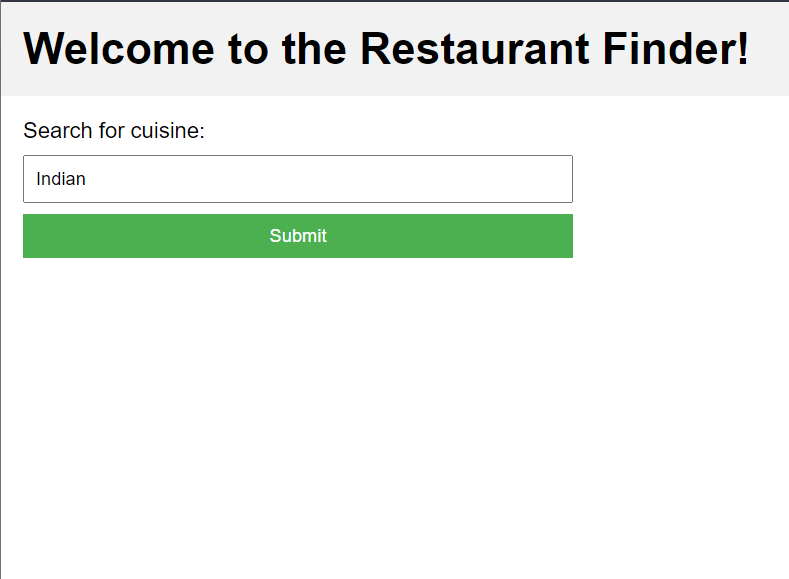
\includegraphics[scale = 0.4]{images/IndianQ.png}
    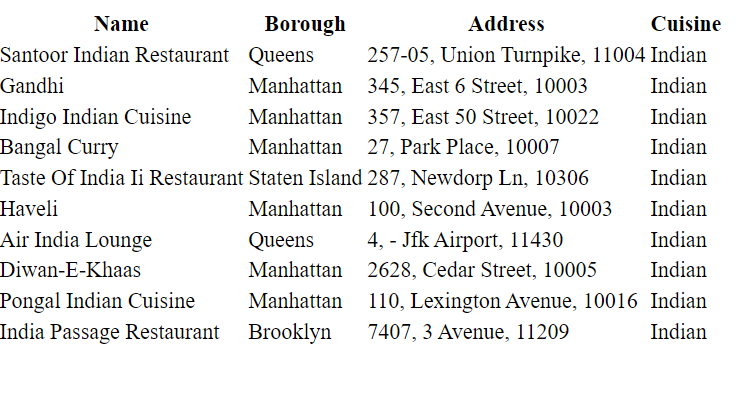
\includegraphics[scale = 0.4]{images/IndianList.png}
    \caption{Search Restaurants with Indian Cuisine}
\end{figure}

\begin{figure}[h!]
    \centering
    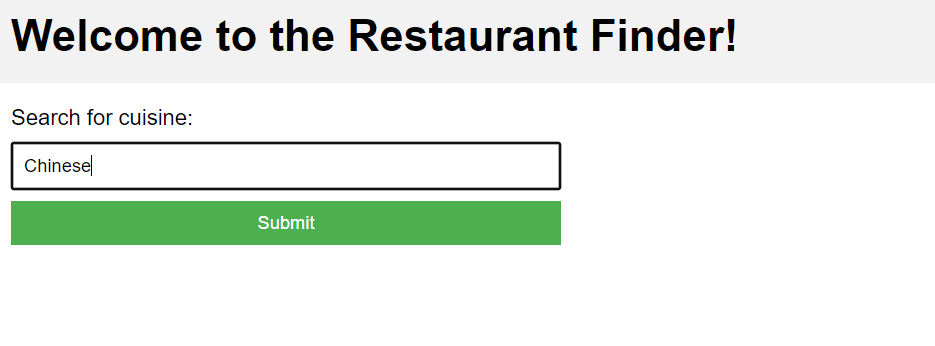
\includegraphics[scale = 0.4]{images/ChineseQ.png}
    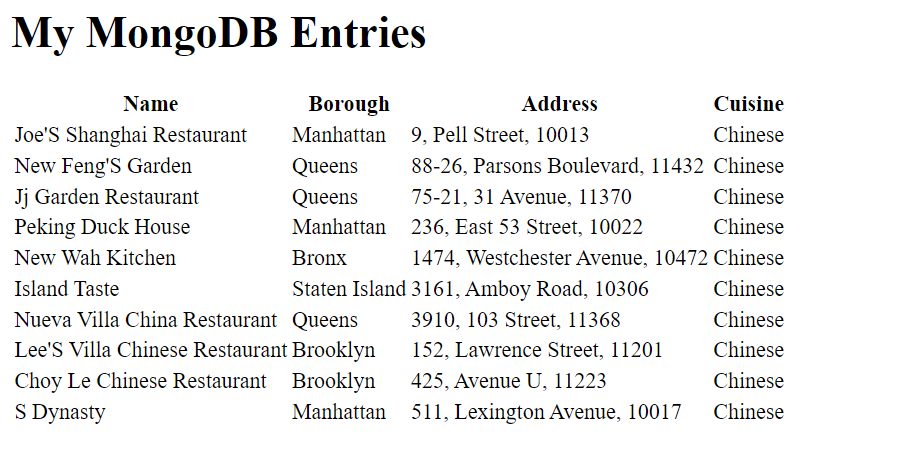
\includegraphics[scale = 0.4]{images/ChineseList.png}
    \caption{Search Restaurants with Chinese Cuisine}
\end{figure}

\begin{figure}[h!]
    \centering
    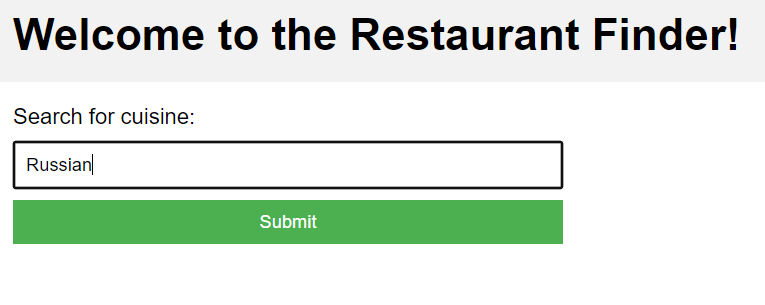
\includegraphics[scale = 0.6]{images/RussianQ.png}
    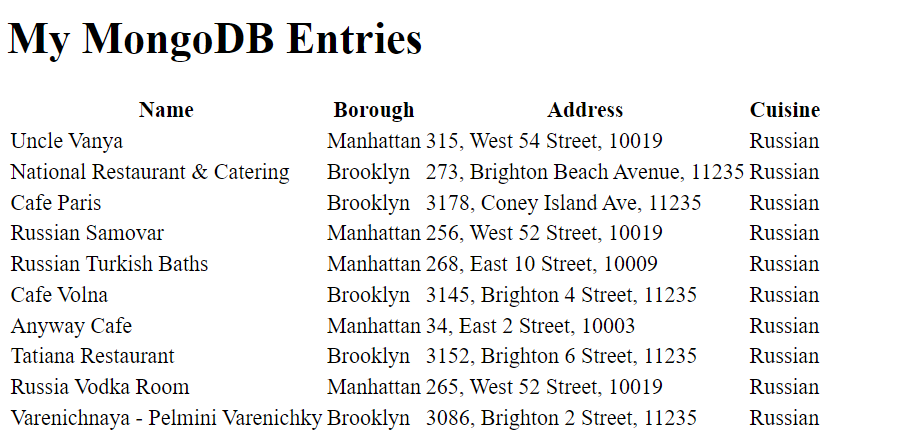
\includegraphics[scale = 0.6]{images/RussianList.png}
    \caption{Search Restaurants with Russian Cuisine}
\end{figure}
\pagebreak
\section{Conclusion}
This restaurant finder application is a useful tool for users looking to discover new restaurants based on cuisine preferences. The Elasticsearch index ensures that search queries are fast and accurate, while the MongoDB database provides a reliable source of restaurant data. The simple and user-friendly design of the application allows for easy navigation and a positive user experience. Overall, this project successfully demonstrates the use of Elasticsearch and MongoDB in a Flask application for finding restaurants by cuisine.

\section{Appendix}
\appendix
\section{Project Link}
https://github.com/bishal216/RandomStuffs/tree/main/BigData/Project

\section{MongoDB data sample}
\begin{table}[h!]
    \centering
    \begin{tabular}{lllll}
        \hline
        \textbf{Cuisine} & \textbf{Name} & \textbf{Borough} & \textbf{Address} & \textbf{...} \\ \hline
        American & The Capital Grille & Manhattan & 120 W 51st St & ... \\
        Chinese & Joe's Shanghai & Queens & 136-21 37th Ave & ... \\
        Italian & Carbone & Manhattan & 181 Thompson St & ... \\
        Japanese & Sushi Yasuda & Manhattan & 204 E 43rd St & ... \\
        Mexican & Cosme & Manhattan & 35 E 21st St & ... \\
        Pizza & Di Fara Pizza & Brooklyn & 1424 Ave J & ... \\
        Thai & SriPraPhai & Queens & 64-13 39th Ave & ... \\
        Vegetarian & Dirt Candy & Manhattan & 86 Allen St & ... \\ \hline
        \end{tabular}
        \caption{Sample Data from MongoDB}
    \end{table}
    \section{Elasticsearch index Mapping}
    \begin{table}[h!]
        \centering
        \begin{tabular}{ llll } 
         \hline
         \textbf{Field} & \textbf{Data Type} & \textbf{Index} & \textbf{Description} \\
         \hline
         name & text & analyzed & Name of the restaurant \\
         \hline
         cuisine & text & analyzed & Type of cuisine served \\
         \hline
         borough & text & analyzed & Borough in which the restaurant is located \\
         \hline
         address & text & analyzed & Address of the restaurant \\
         \hline
         rating & float & not analyzed & Rating of the restaurant on a scale of 1-5 \\
         \hline
         price & integer & not analyzed & Price level of the restaurant (1-4) \\
         \hline
         location & geo\_point & not analyzed & Latitude and longitude of the restaurant \\
         \hline
        \end{tabular}
        \caption{Elasticsearch index mapping for restaurant data}
        \label{table:elasticsearch-index-mapping}
        \end{table}
\end{document}